\section{Model Predictive Control}
\label{sec:mpc}
Following the identification of the model done in section \ref{sec:trajectory_optimization}, an optimal control strategy was developed for the deployment of the zone heating by means of model predictive control (MPC). First, a primal optimal problem was developed for the MPC application which resulted in a significant decrease in energy consumption and therefore energy costs. Nevertheless, due to the constraint nature of primal optimal problems, the robustness of the control was a matter of concern. Due to this, a second approach following a lagrangian problem statement was developed. This allowed for the relaxation of the constraints, leading to a more robust control. The details pertaining both approaches are thoroughly explained in their corresponding subsections in the following.

\subsection{Primal MPC}
\label{subsec:primal_mpc}
As a first step, the calculated constants from section \ref{sec:trajectory_optimization} were used to develop the model. In order to ensure a proper MPC development, model state and control variables were determined. For this, the zone temperature $T_z$, ambient temperature $T_a$, solar radiation $\dot{Q}_{sun}$ and the heat input due to occupancy $\dot{Q}_g$ were taken as the system states $\boldsymbol{X}$. Since the goal of the MPC is the optimal deployment of the zone heating $\dot{Q}_{h}$, it was taken as the control variable $U$. The following code shows how these were expressed.

\begin{python}
    # Constants
    N = len(time)  # Number of samples
    delta_t = 3600  # [s] in 1 hour
    nx = 4  # Number of states for system
    
    # Taking the optimal parameters calculated
    R = R_opt
    C = C_opt
    gA = gA_opt

    # Initializing optimization problem
    opti = Opti()
    X = opti.variable(nx, N + 1)  # states: Tz [K], Ta [K], Qsun [W/m2], Qg [W]. Multiple shooting

    U = opti.variable(N, 1)  # control variable: Qh [W]
\end{python}

Here, it can be seen that the state variable vector is initialized as a 4 by N+1 vector. This is since the transcription method used during this optimization is multiple shooting, which requires an additional state instance when compared to the control vector.\\

Moreover, the state vector was filled by means of a for-loop, following equation \ref{eq:finite_difference_model} and populating the rest of the states from the data collected in appendix \ref{appendix}.
\begin{python}[basicstyle=\small]
# Setting shooting constraints
for i in range(N - 1):
   opti.subject_to(X[0,i+1] == delta_t * ((X[2,i] * gA + U[i] + X[3,i])/C + (X[1,i]-X[0,i])/(R*C)) + X[0,i])
\end{python}    
\begin{python}
    opti.subject_to(X[1, i + 1] == temp[i + 1])
    opti.subject_to(X[2, i + 1] == Qsun[i + 1])
    opti.subject_to(X[3, i + 1] == Qg[i + 1])
\end{python}

Here, the first state is fully determined as a function of the control values, allowing for the optimization of its deployment. Additionally, the first instance for all states is purposefully skipped since the initial conditions are set at a later stage by means of the initial guess vector $\boldsymbol{X}_0$.\\

Next, the matter of constraints is considered. For this, first the physical limits for the radiator are stated by setting the control variables to be within 0 and 1000 W (its maximal heating output). Furthermore, the thermal comfort limits were placed for the zone temperature for instances on which someone is occupying the zone. This allows for the reduction of heating output during non-occupation times, leading to lower electrical costs. For this, a typical occupational time range was used on which there is one person inside the zone during the entire weekend and the zone is not occupied in the weekdays from 07:00 to 18:00.

\begin{python}
# Setting bounded constraints (temp range for the zone whenever someone is home)
opti.subject_to(opti.bounded(293.15, X[0, 0:24], 298.15))  # Weekend
opti.subject_to(opti.bounded(293.15, X[0, 144:], 298.15))  # Weekend
for i in range(6):  # Weekdays
   opti.subject_to(opti.bounded(293.15, X[0,0+24*(i+1):7+24*(i+1)], 298.15))
   opti.subject_to(opti.bounded(293.15, X[0,18+24*(i+1):24+24*(i+1)], 298.15))

# Bounded constraints for max and min power output for the radiator
opti.subject_to(opti.bounded(0, U, 1000))
\end{python}

Next, initial conditions as well as the objective function were stated. Since the goal of the MPC is the reduction of energy consumption, the squared sum of the total heat deployed into the zone via the radiator $\sum \dot{Q}_{h}^2$ was declared as the cost function. The following snippet illustrates how both were introduced into CasADi.

\begin{python}
# Setting initial conditions
opti.subject_to(X[:, 0] == x0)

# Setting minimization equation
opti.minimize(sumsqr(U))

opti.set_value(x0, vertcat(293.15, temp[0], Qsun[0], Qg[0]))

opti.solver('ipopt')
sol = opti.solve()
\end{python}

The optimal control problem is then ready to be solved by means of the IPOPT solver. In order to provide more clarity, equations \ref{eq:mpc1} to \ref{eq:mpc2} summarize the above stated code in equation form.


\begin{equation}
{\text{minimize}} \hspace{1em} \sum_{i=1}^{N} \left(\dot{Q}_{h,i}\right)^2
\label{eq:mpc1}
\end{equation}
\begin{equation}
\text{subject to}  \hspace{1em} T_{z,i+1} - \Delta t \left( \frac{\dot{Q}_{h,i} + gA \cdot \dot{Q}_{sun, i} + \dot{Q}_{g,i}}{C_z} + \frac{T_{z,i}-T_{a,i}}{R_w \cdot C_z} \right) - T_{z,i} =0
\end{equation}
\vspace{-0.5em}
\begin{align}
\left[T_{z,0}, T_{a,0}, \dot{Q}_{sun,0}, \dot{Q}_{g,0}\right]^{\top}  - \boldsymbol{X}_0 &=  0 \\[0.5em]
T_{z,i} - 298.15 &\leq 0 \hspace{2em} \forall i \in \text{occupied}\\[0.5em]
293.15 - T_{z,i} &\leq 0 \hspace{2em} \forall i \in \text{occupied}\\[0.5em]
\dot{Q}_{h,i} - 1000 &\leq 0\\[0.5em]
-\dot{Q}_{h,i} &\leq 0
\label{eq:mpc2}
\end{align}

Lastly, the above stated MPC results in the temperature and heating deployment profiles seen in Figure \ref{fig:mpc_primal}.

\begin{figure}[H]
\centering
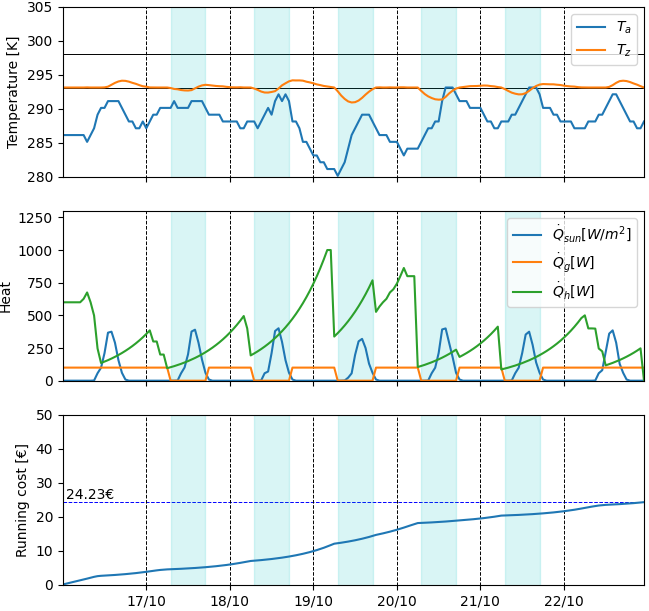
\includegraphics[scale=0.8]{images/mpc_primal.png}
\caption{MPC by means of a primal optimal problem for the zone heat deployment.}
\label{fig:mpc_primal}
\end{figure}

Immediately, when comparing Figures \ref{fig:mpc_primal} and \ref{fig:onoff_radiator} a decrease in weekly cost of about 42\% can be seen. Additionally, this cost reduction comes with a more stable temperature profile for the zone, ensuring thermal comfort at all occupant times. It can also be noted that the heat deployment is maintained well below the maximum power output for most days, helping towards the reduction of energy use and the extension of the lifespan of the radiator.\\

While appreciating the benefits of the integrated MPC, the issue of robustness raises a large concern for the application of this system. This is due mainly to the strictness of the constraints for the zone temperature profile. By introducing the thermal comfort boundaries for the zone as a bounded constraint, we do not allow for considerations of exterior influences causing a drastic change in zone temperature and taking the zone outside of its comfort range (e.g. an open window, sudden rain, etc.). This effect is easily tested by varying the initial temperature from 293.15 $\mathsf{K}$ to 283.15 $\mathsf{K}$. This change on the initial vector, quickly backs the hypothesis since, by enforcing a temperature outside of the thermal comfort range, the solver is unable to return a solution and instead gives the error \texttt{return\_status is `Infeasible\_Problem\_Detected'}.\\

For this reason, it was decided that these constraints should be relaxed in order to increase the robustness of the system. This is done by introducing a penalty variable into the cost function, which is developed in the following subsection.

\newpage
\subsection{Relaxed MPC}
\label{subsec:relaxed_mpc}
Considering the robustness issues discussed in subsection \ref{subsec:primal_mpc}, a relaxed approach was taken. For this, the same initial steps were taken as before. The distinction between both approaches is seen during the constraints setting portion of the code. When taking a relaxed approach, an additional slack variable is introduced into the control vector. 

\begin{python}
# Initializing optimization problem
opti = Opti()

X = opti.variable(4, N)  # States: Tz [K], Ta [K], Qsun [W/m2], Qg [W].

U = opti.variable(N, 2)  # Qh [W] and slack variable S [-]
\end{python}

This slack variable $S$ is then introduced into the cost function alongside a penalty factor as well as into the inequality constraints in order to allow for a larger flexibility for the system. Figure \ref{fig:relaxed_mpc_st} shows this integration of the slack variable in the form of a control variable.

\begin{figure}[H]
\centering
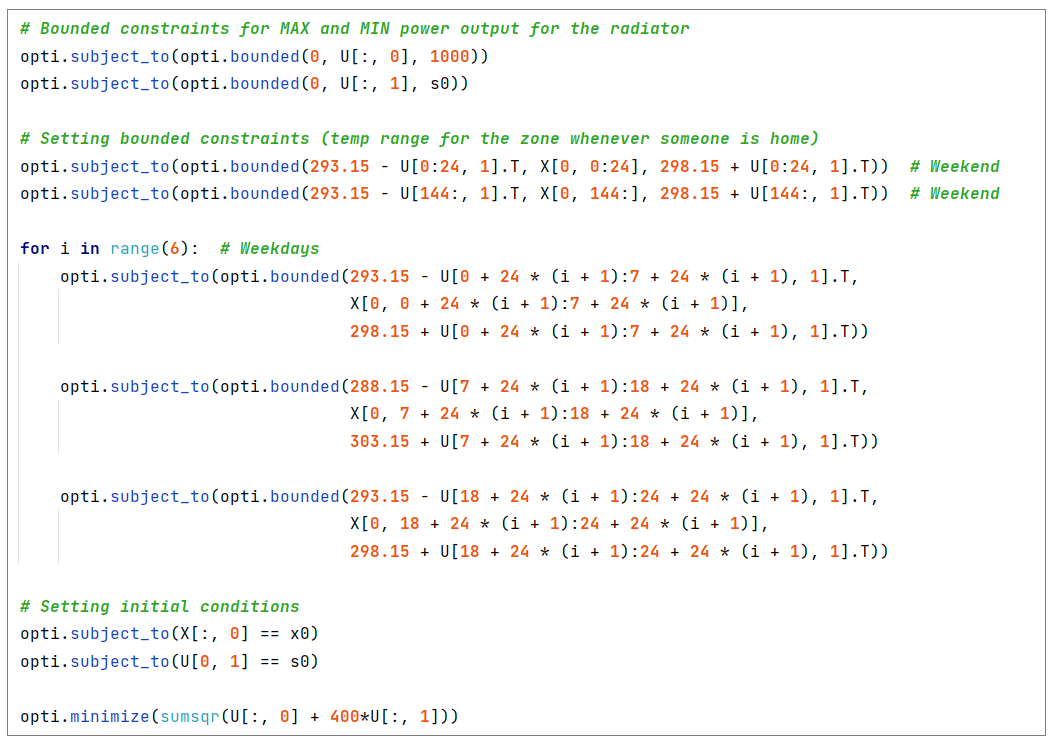
\includegraphics[width=\textwidth]{images/relaxed_mpc_st2.png}
\caption{Integration of slack variable $S$ (here \texttt{U[:, 1]}) into thermal comfort limits.}
\label{fig:relaxed_mpc_st}
\end{figure}

A few things can be mentioned here. First, the constraints for the zone heating $Q_h$ (here \texttt{U[:, 0]}) remain the same as the previous primal case. This is because the heater limits must be set as hard constraints since it is unphysical for the equipment to go beyond its maximum heating output. Moreover, it can be seen that limits are set for the slack variable. In particular, they are set to be between 0 and an initial value $s_0$ which is usually in the order of $10^5$. It is common practice to set this initial value to be very large in order to allow enough flexibility for the system to adjust itself in the initial instance. It can be seen that this value decreases rapidly as the OCP attempts to reach the set temperature ranges. \\

Next, the thermal comfort ranges are set. For this, the slack variable is introduced such that instead of the inequality constraints are set to be $\leq 0$, they are set to be $\leq S$. This allows for the system to not become unfeasible in the case where the comfort limits are breached. Additionally, instead of removing the constraints whenever someone is not home, the thermal comfort range is widened (seen in Figure \ref{fig:relaxed_mpc_st} in the second command within the \texttt{for} loop) from [293.15, 298.15] to [288.15, 303.15]. This allows for a reduction in heat consumption while not allowing for the zone temperature to drop too much and hinder the comfort for the following occupancy period.\\


%Here, the introduction of the lagrange multipliers $\boldsymbol{\mu}_1$ and $\boldsymbol{\mu}_2$ can be seen for the upper and lower thermal comfort boundaries, respectively. By varying these values, their weight (or importance) within the cost function varies, therefore these must be tuned depending on the preferences of the user. In the case lowering energy use is considered to be of highest importance, lower $\boldsymbol{\mu}_i$ values would be used. On the other hand, if thermal comfort during occupancy times is the priority, higher $\boldsymbol{\mu}_i$ values would be introduced. For the application shown here, a relative balance was attempted between both objectives: a maintenance of thermal comfort while taking into consideration energy use. Moreover, in order to account for `at work' hours, the lagrangian multiplier values were decreased by 20\% during those instances in order to reduce energy use while still allowing for the zone to pre-heat itself whenever someone is expected to come home.\\

Finally, the cost function is declared as before with the addition of the slack variable multiplied by a penalty factor (here = 400). This factor must be tuned according to the preferences of the user. A larger factor gives a larger penalty to the zone crossing the thermal comfort limits, resulting in a more constant zone temperature at the cost of higher energy consumption. The opposite case is true for smaller penalty factors. This value was achieved by tuning to an appropriate balance between both, although, as mentioned, this balance is user-dependent.\\

The resulting optimal control problem can be stated mathematically as the following:

\begin{equation}
{\text{minimize}} \hspace{1em} \sum_{i=1}^{N} \left(\dot{Q}_{h,i} + 400\cdot S_i\right)^2
\label{eq:mpclag1}
\end{equation}
\begin{equation}
\text{subject to}  \hspace{1em} T_{z,i+1} - \Delta t \left( \frac{\dot{Q}_{h,i} + gA \cdot \dot{Q}_{sun, i} + \dot{Q}_{g,i}}{C_z} + \frac{T_{z,i}-T_{a,i}}{R_w \cdot C_z} \right) - T_{z,i} =0
\end{equation}
\vspace{-0.5em}
\begin{align}
\left[T_{z,0}, T_{a,0}, \dot{Q}_{sun,0}, \dot{Q}_{g,0}\right]^{\top}  - \boldsymbol{X}_0 &=  0 \\[0.5em]
S_0 &= 10^5 \\[0.5em]
T_{z,i} - 298.15 &\leq S_i \hspace{2em} \forall i \in \text{occupied}\\[0.5em]
293.15 - T_{z,i} &\leq S_i \hspace{2em} \forall i \in \text{occupied}\\[0.5em]
T_{z,i} - 303.15 &\leq S_i \hspace{2em} \forall i \notin \text{occupied}\\[0.5em]
288.15 - T_{z,i} &\leq S_i \hspace{2em} \forall i \notin \text{occupied}\\[0.5em]
\dot{Q}_{h,i} - 1000 &\leq 0\\[0.5em]
-\dot{Q}_{h,i} &\leq 0
\label{eq:mpclag2}
\end{align}

Finally, the results for this optimal control problem can be seen in Figure \ref{fig:mpc_lagrangian}.

\begin{figure}[H]
\centering
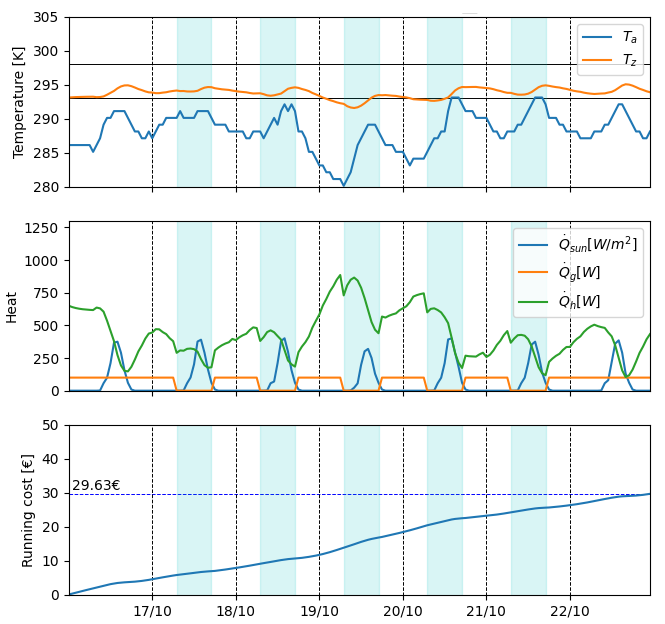
\includegraphics[scale=0.8]{images/mpc_lagrangian.png}
\caption{MPC by means of a relaxed optimal control problem for the zone heat deployment.}
\label{fig:mpc_lagrangian}
\end{figure}

Comparing these results to Figure \ref{fig:onoff_radiator}, Figure \ref{fig:mpc_lagrangian} shows a further decrease in energy costs when compared to Figure \ref{fig:mpc_primal}. Here, a 49\% cost reduction can be observed when compared to the baseline case. These savings surpass the already high savings seen in the primal MPC application (42\%) while having a much more robust behavior.\\

More significantly, this MPC application follows reality more accurately than the one developed using a primal problem statement. By not forcing the zone temperature to be within the comfort boundaries at all moments, the system becomes robust towards outliers and sudden changes caused by third parties without crashing. Figure \ref{fig:mpc_lagrangian_Tstart} shows the results for the same experiment done in subsection \ref{subsec:primal_mpc} starting from 283.15 K. Here, the robustness of the relaxed problem statement becomes evident since, by removing the hard constraints, the system allows for outliers without crashing while still penalizing them and quickly recovering.

\begin{figure}[H]
\centering
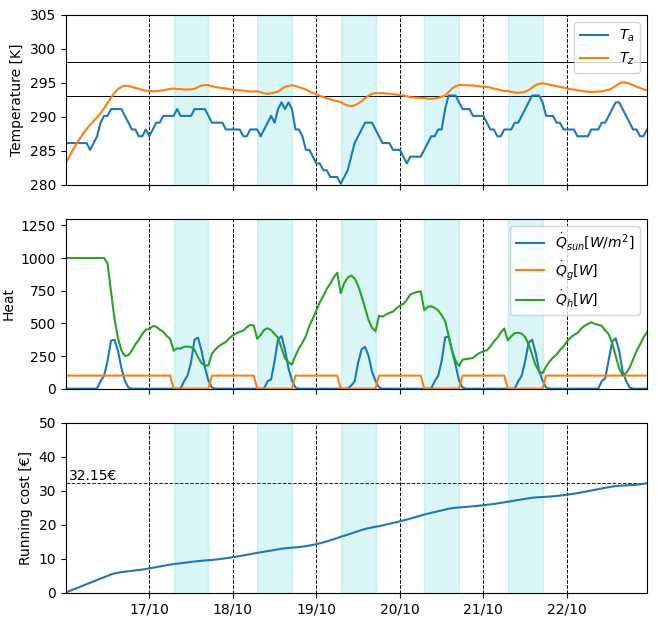
\includegraphics[scale=0.8]{images/mpc_lagrangian_Tstart.png}
\caption{MPC by means of a lagrangian optimal problem for the zone heat deployment with deviated initial zone temperature.}
\label{fig:mpc_lagrangian_Tstart}
\end{figure}